En esta seccion se describen brevemente distintos enfoques software tanto a nivel de planificadores de tareas
en tiempo de ejecución como de bibliotecas matemáticas, específicamente desarrollados para arquitecturas 
asimétricas (o heterogéneas).

\section{Planificación en tiempo de ejecución de operaciones complejas}

\subsection{Planificación de tareas en la Factorización de Cholesky}

A continuación describimos los mecanismos utilizados para extraer paralelismo a nivel de tareas
durante la ejecución de una operación específica de álgebra lineal densa, utilizando la Factorización
de Cholesky como hilo conductor. Esta operación en particular es representativa de muchas
otras factorizaciones utilizadas en la resolución de sistemas lineales, por lo que gran parte de las
conclusiones extraídas sobre ella pueden ser aplicadas a otro tipo de operaciones similares ampliamente
utilizadas en ciencia e ingeniería.
%
La Factorización de Cholesky descompone una matriz simétrica definida positiva
$A$ en el producto $A=U^TU$, donde el factor de Cholesky $U$ de dimensión $n \times n$ $U$ es una matriz triangular
superior~\cite{GVL3}. 

\lstinputlisting[float=th!,frame=lines,caption=Implementación en lenguaje C de la factorización de Cholesky orientada a bloques.,label=lst:chol]{Codes/cholesky.c}

El código de la Figura~\ref{lst:chol} muestra un código simplificado en lenguaje C para
la factorización de una matriz {\tt A} de dimensiones {\tt n}$\times${\tt n}, 
almacenada como un conjunto de {\tt s}$\times${\tt s} submatrices (bloques de datos) de dimensíón 
{\tt b}$\times${\tt b}.

Esta rutina orientada a bloques descompone la operación global en una colección de kernels u operaciones
fundamentales:
{\tt po\_cholesky} (Factorización de Cholesky), {\tt tr\_solve} (resolución de un sistema triangular),
{\tt ge\_multiply} (multiplicación de matrices), y 
{\tt sy\_update} (actualización simétrica de rango-{\tt b}), que operan sobre cada bloque
de datos de la matriz, y forman parte de las rutinas proporcionadas por los estándares LAPACK y BLAS. 

\begin{figure}%[tbh!]
\begin{center}
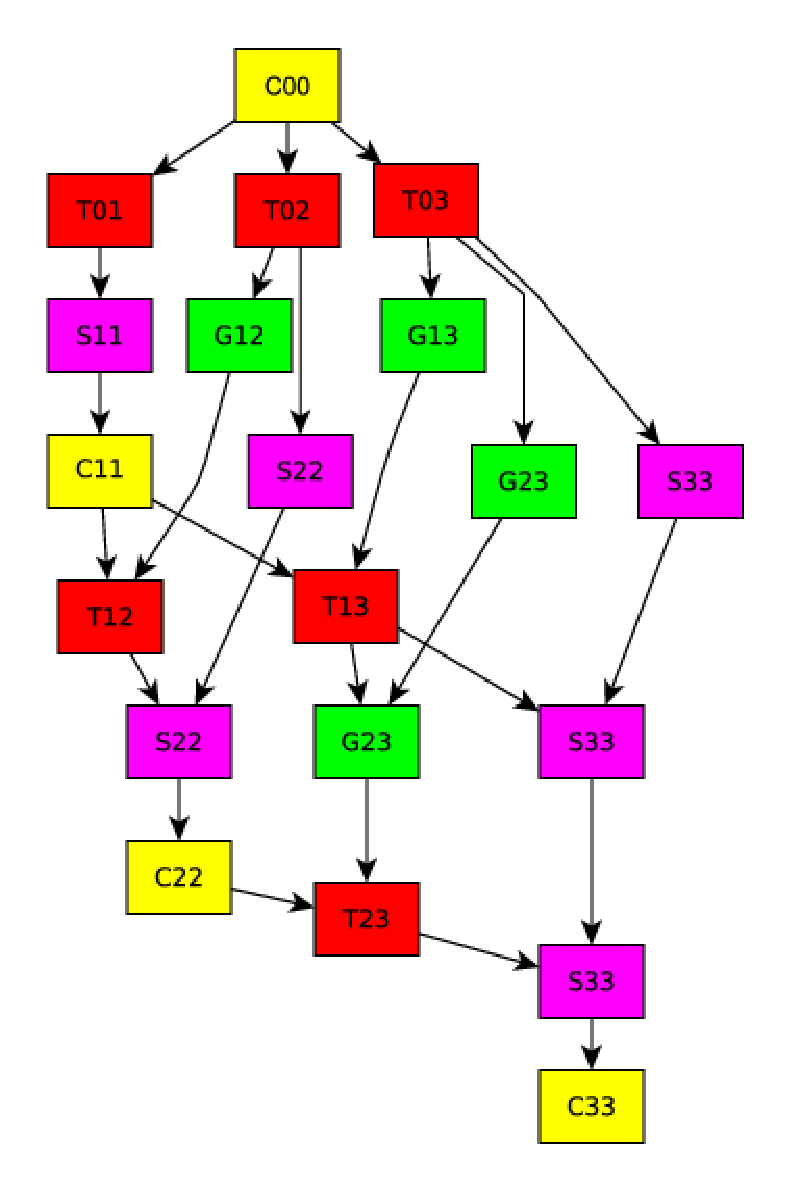
\includegraphics[scale=0.35]{Figures/4x4_TaskExample}
\end{center}
\caption{DAG con las tareas y dependencias de datos resultantes de la aplicación del código en la Figura~\ref{lst:chol}
         sobre una matriz compuesta por $4 \times 4$ bloques ({\tt s}=4). Las etiquetas especifican el tipo de kernel/tarea
         con la siguiente correspondencia: 
         ``{\sf C}'' para la Factorización de Cholesky,
         ``{\sf T}'' para la resolución de sistema triangular,
         ``{\sf G}'' para la multiplicación de matrices, y
         ``{\sf S}'' para la actualización simétrica de rango-{\tt b}. 
	 Los subíndices (comenzando en 0) especifican la submatriz que la tarea correspondiente actualiza.}
\label{fig:dag}
%\vspace{-0.5cm}
\end{figure}

El orden en el que dichos kernels son invocados durante la ejecución de la rutina, 
así como las submatrices o bloques que cada kernel lee o escribe, genera un grafo acíclico dirigido (DAG)
que refleja las dependiencias entre tareas (esto es, entre instancias de los kernels) y, por tanto,
el paralelismo de tareas potencial de la operación.
Por ejemplo, la Figura ~\ref{fig:dag} muestra el DAG con las tareas (nodos) y las dependencias de datos
(arcos) intrínsecas a la ejecución del código de la Figura~\ref{lst:chol}, cuando éste se ejecuta sobre
una matriz compuesta por $4 \times 4$ submatrices (esto es, cuando {\tt s}=4).  

\section{Modelos de programación basados en paralelismo a nivel de tareas}

El DAG asociado con un algoritmo o rutina es una representación gráfica del paralelismo de tareas asociado a ella,
e, idealmente, un planificador de tareas en tiempo de ejecución podría explotar esta información para determinar
distintas planificaciones (esto es, ordenación de tareas y asignación de las mismas a recursos computacionales
disponibles) que satisfacen las dependencias fijadas en el DAG.

\subsection{Modelo de programación y planificación de tareas en OmpSs}

Con el fin de ayudar al programador en la construcción de un DAG completo y correcto partiendo de un código secuencial,
modelos de programación como OmpSs proporcionan mecanismos sencillos y no invasivos. En dicho modelo, el programador 
utiliza directivas similares a OpenMP ({\tt pragma}s) para anotar rutinas existentes en el código como tareas, indicando
a la vez la direccionalidad de sus operandos (entrada, salida o entrada/salida) a través de cláusulas adicionales. A 
grandes rasgos, el planificador de OmpSs descompone el código (transformado previamente a través del compilador 
fuente-a-fuente Mercurium~\cite{Mercurium}) en un conjunto de tareas, identificando las dependencias entre ellas, 
y lanzando a ejecución únicamente {\em tareas listas} (es decir, aquellas cuyas dependencias han sido satisfechas)
para su ejecución en los distintos núcleos computacionales del sistema.


El código de la Figura~\ref{lst:chol_tasks} muestra las anotaciones necesarias por parte del programador para explotar
el paralelismo a nivel de tareas inherente a la factorización de Cholesky usando OmpSs; cabe destacar las líneas etiquetadas
con  anotaciones (directivas) ``{\tt \#pragma omp}''.
Las cláusulas {\tt in}, {\tt out} e {\tt inout} denotan la direccionalidad de los datos, y ayudan al planificador
de tareas a mantener coherentemente las dependencias entre tareas durante la ejecución. 
En esta implementación, los cuatro kernels anotados son implementados como invocaciones a 
kernels computacionales básicos de álgebra lineal proporcionados por LAPACK
({\tt dpotrf}) y BLAS ({\tt dtrsm}, {\tt dgemm} y {\tt dsyrk}).

\lstinputlisting[float=th!,frame=lines,caption=Tareas etiquetadas necesarias para la factorización de Cholesky por bloques.,label=lst:chol_tasks]{Codes/cholesky_tasks.c}

\subsection{Adaptación de OmpSs a arquitecturas asimétricas (botlev)}
\label{s3:botlev}

En servidores equipados con uno o más aceleradores --por ejemplo, procesadores gráficos--, versiones especializadas de los
planificadores de tareas que acompañan a OmpSs, StarPU, MAGMA, Kaapi y {\tt libflame} (añadir referencias!!) son capaces
de planificar tareas a núcleos de propósito general (CPUs en adelante) o a aceleradores (por ejemplo, procesadores gráficos
--GPUs-- o Intel Xeon Phi), asignando tareas a cada tipo de recurso en función de sus propiedades, y aplicando técnicas
como caches gestionadas por software o mapeado de tareas explotando la localidad de datos (véanse, entre 
otros,~\cite{Quintana:2008:PMA,CPE:CPE1463,Augonnet:2011:SUP:1951453.1951454,5470941,Gautier:2013:XRS:2510661.2511383}. Este
tipo de adaptaciones, además, permiten la gestión transparente de transferencias de datos entre distintos espacios de 
memoria, característica principale en sistemas heterogéneos modernos.

%Recently OmpSs has been extended with a tailored scheduler for ARM big.LITTLE processors that 
%discriminates between the target being a fast (big) or a slow (LITTLE) core. This variant integrates uni- or bi-directional
%work stealing between the two types of cores, and specific criticality-aware mapping techniques~\cite{OmpSsbigLITTLE}. This runtime will be
%used as a base of our comparative experimental analysis in the experiments.

%%
\comentario{Título: No se si adaptación, o ampliación, o incorporación, o uso de
  OmpSs sobre asim, o ...} %%
Con el reciente auge de las arquitecturas asimétricas en el mundo HPC, el
equipo de desarrollo de OmpSs ha introducido un nuevo planificador
denominado \emph{Bottom level-aware scheduler} (Botlev)~\cite{botlev}
específico para este nuevo tipo de arquitecturas. Botlev recoge las ideas
de los planificadores tradicionales basados en arquitecturas heterogéneas,
distinguiendo únicamente dos tipos de nodos de cómputo (un nodo rápido
formado por los cores de tipo big, y un nodo de cómputo lento formado por
los cores de tipo LITTLE) y eliminando el
cálculo de los costes asociados a la transferencia de datos. \\
La principal idea que se encuentra detrás de Botlev es la de detectar en
tiempo de ejecución qué tareas pertenecen al camino crítico y cuáles no, y
obligar a que los cores rápidos sean los encargados de ejecutar las tareas
del camino crítico. Además, en caso de existir alguna tarea perteneciente
al camino crítico lista para ser ejecutada, esta tendrá preferencia sobre
el resto de tareas que también estén listas para ejecución.\\
El objetivo de garantizar que las tareas del camino crítico se ejecutan en
los cores rápidos cuanto antes es asegurarse que al ejecutar las tareas
críticas, estas liberarán dependencias con nuevas tareas que pasarán a
estar listas para ejecución, y así intentar conseguir que nunca haya cores
ociosos, lo cual disminuiría el rendimiento global de la aplicación. La
principal diferencia entre botlev y los planificadores tradicionales para
sistemas heterogéneos es que botlev toma las decisiones en tiempo dinámico
sin necesidad de conocer de antemano información sobre las tareas, o al
forma del árbol de dependencias.

Para determinar si una tarea pertenece al camino crítico o no en tiempo de
ejecución, botlev asigna una prioridad a cada tarea en el momento de la
inserción en el grafo de dependencias. Una vez que la tarea está lista para
ser ejecutada (es decir, cuando todas las tareas que tenían relación con la
tarea mediante el grafo de dependencias han finalizado su ejecución), se
realiza la decisión de qué core va a ejecutar la tarea en función de la
prioridad
asignada.\\
La prioridad de una tarea viene dada por un número entero positivo, el cuál
representa la longitud del camino más largo desde la tarea actual hasta una
tarea hoja del grafo de dependencias. Cuando una tarea es introducida en el
grafo de dependencias, se le asigna una prioridad 0 ya que la longitud del
camino más largo desde la tarea a un nodo hoja (ella misma) es 0. Además,
cuando una tarea se inserta en el TDG, se actualizan las prioridades de
todas las tareas predecesoras, ya que estas pueden haber cambiado. Por cada
tarea predecesora, se intenta aumentar la prioridad en 1 unidad (el camino
es un nodo más largo), siempre que no tuviera una prioridad mayor antes
(este es el caso de que la tarea pertenezca a un camino más largo en el que
la nueva tarea no esté involucrada). El proceso de actualización finaliza
cuando se actualiza la tarea raíz del árbol, o cuando se alcanza una tarea
que pertenece a otro camino más largo que el actual. En la
figura~\ref{s3:fig:botlev_tdg} se puede ver el camino crítico detectado
para una factorización de Cholesky sobre una matriz dividida en $8\times8$
bloques. Hay que destacar que esta forma de calcular el camino crítico
detecta las tareas que pertenecen al camino más largo, pero eso no implica
que sean aquellas que más van a retrasar la ejecución en caso de que no se
ejecuten de manera prioritaria. Para calcular esto, sería necesario conocer
de antemano las necesidades de cada tarea, o ir almacenando resultados
parciales de ejecución de manera dinámica para tomar decisiones en el
futuro.
%%
\comentario{La figura de las colas no se ve muy bien.} %%
\begin{figure}
  \centering
  
  \begin{subfigure}{.45\textwidth}
    \centering
    \setlength{\fboxsep}{5pt}
    \fbox{\includegraphics[width=.8\linewidth]{Figures/botlev-tdg.png}}
    \caption{Camino crítico en botlev para una factorización de Cholesky de
      $8\times8$ bloques.}
    \label{s3:fig:botlev_tdg}
  \end{subfigure}
  % Si se deja una línea en blanco, las coloca en vertical
  \begin{subfigure}{.47\textwidth}
    \centering
    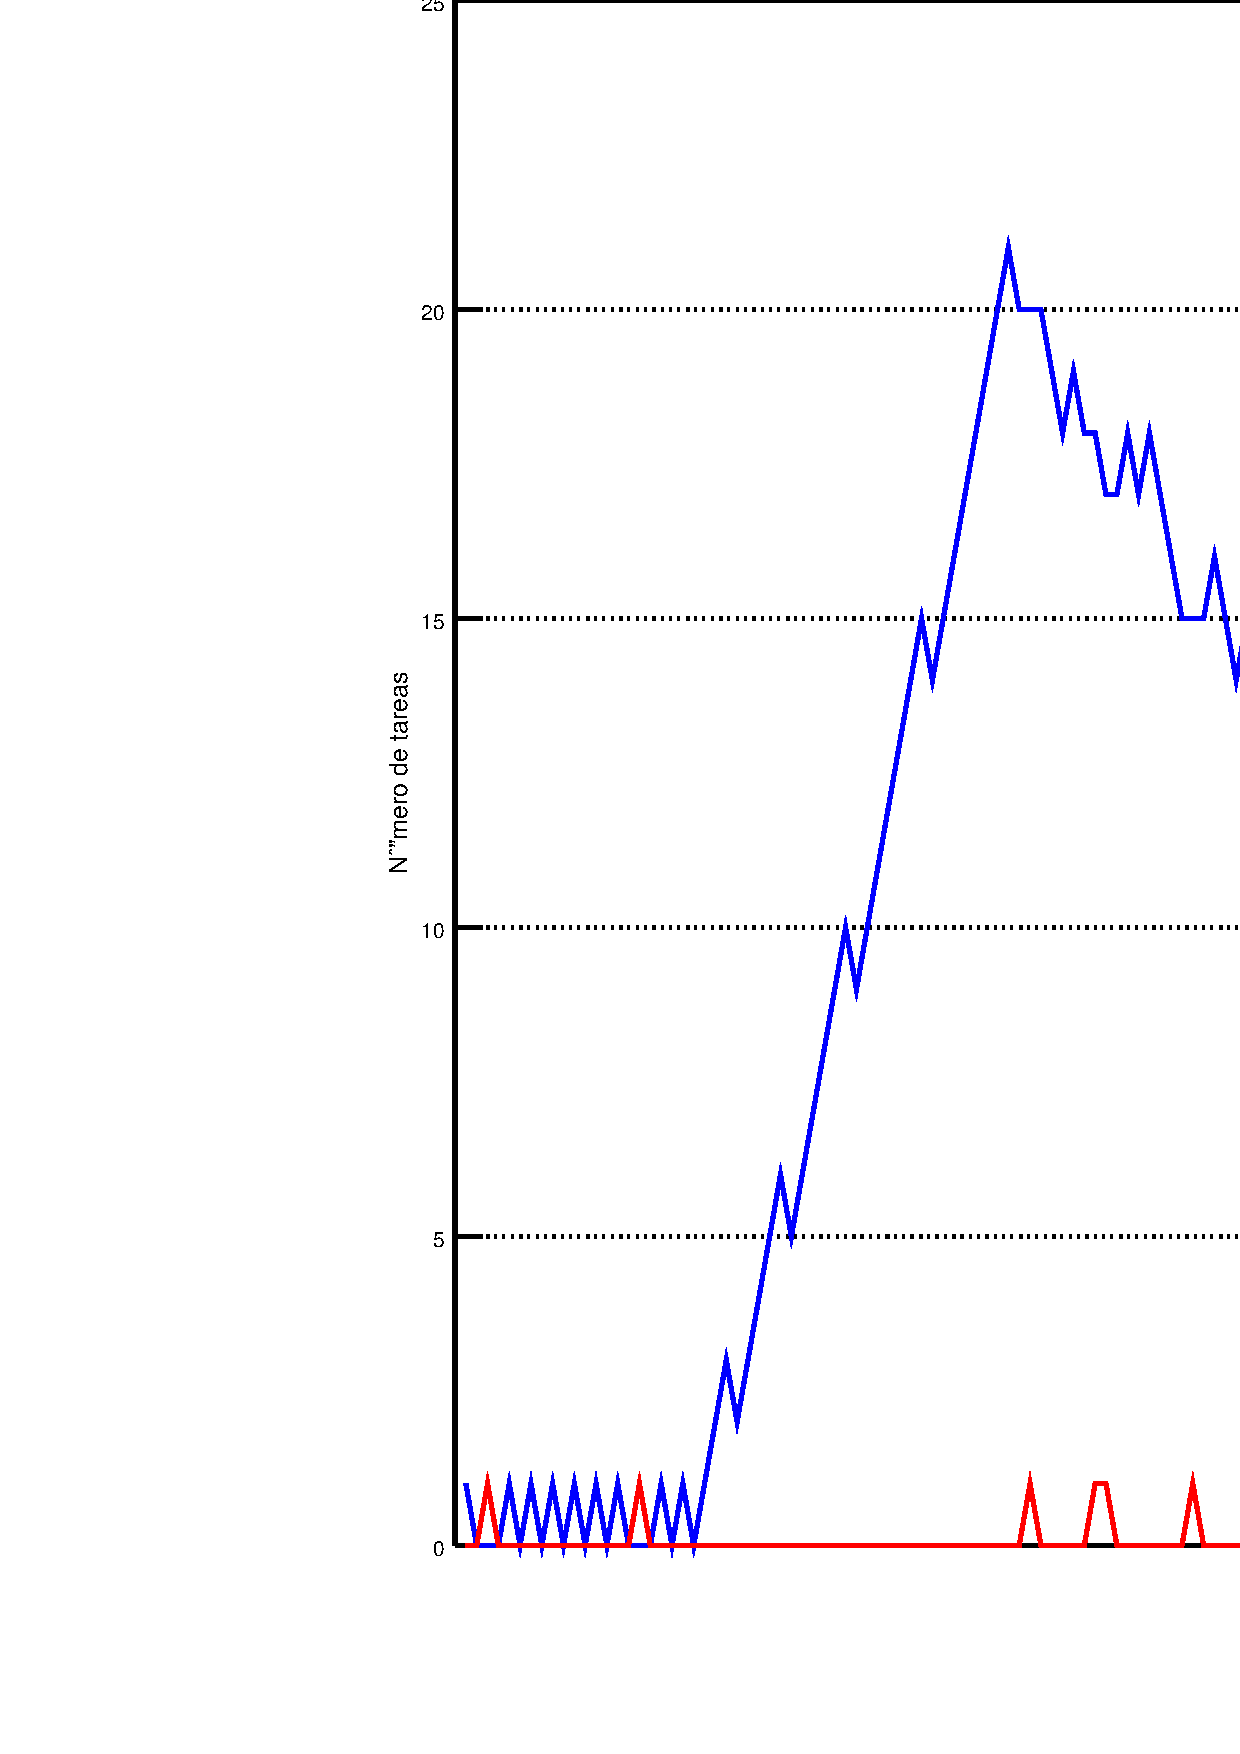
\includegraphics[width=1\linewidth]{Figures/botlev-colas.png}
    \caption{Evolución del tamaño de las colas de tareas
      listas.}
    \label{s3:fig:botlev_colas}
  \end{subfigure}  
  
  \caption{Cálculo de tareas críticas en Botlev y asignación a cores.}
  \label{s3:fig:botlev}
\end{figure}

Una tarea puede ser ejecutada cuando todas sus tareas predecesoras han
finalizado la ejecución. Cuando esto ocurre, Botlev inserta la tarea en una
cola de tareas pendientes para ir ejecutándolas en función de la prioridad
asignada, o en orden de insercción en caso de empate. Estas tareas son
asignadas a los diferentes cores según vayan finalizando la ejecución de
las tareas previas. Según la prioridad de la tarea, Botlev distingue dos
tipos de colas en las que insertar una tarea: la cola con las tareas
pertenecientes al camino crítico, y la cola con el resto de tareas. Una
tarea se considera que pertenece al camino crítico si posee una prioridad
mayor a cualquiera de las prioridades de las tareas anteriores, o si es
hija directa de una tarea que se ha considerado crítica y tiene una
prioridad de una unidad menor (es decir, es el siguiente nodo del camino
crítico). En la figura~\ref{s3:fig:botlev_colas} se puede ver la evolución
del tamaño de las colas para una factorización de Cholesky sobre una matriz
de $16\times16$ bloques. La línea azul muestra el número de tareas no
críticas listas para ser ejecutadas en función del momento de la ejecución
del problema, mientras que la línea roja muestra el número de tareas
críticas. Como se puede apreciar del grafo de dependencias, una
factorización de cholesky está caracterizada por un grafo que se expande
muy rápidamente al principio, y va disminuyendo su tamaño poco a poco hasta
finalizar la ejecución. Este comportamiento se refleja también en la
evolución del tamaño de las colas, donde al principio se identifican la
mayoría de tareas como críticas, y una vez que el árbol comienza a
expandirse, el número de tareas críticas cae drásticamente mientras que el
número de tareas no críticas se eleva considerablemente. 

Cuando un core big finaliza la ejecución de una tarea, este ejecutará la
siguiente tarea de la cola de tareas críticas, mientras que un core LITTLE
ejecutará la primera tarea de la cola de tareas no críticas. De esta forma
se consigue asignar las tareas críticas a cores big, mientras que las
tareas no críticas serán ejecutadas por cores lentos. Para grafos de
dependencias muy anchos, como puede ser el asociado a una factorización de
Cholesky, el número de tareas críticas es mucho menor que el número de
tareas no críticas, dando lugar a que los cores rápidos estén la mayor
parte de tiempo ociosos. Para evitar esta situación, si un core big no
dispone de tareas críticas que ejecutar, ejecutará la siguiente tarea de la
lista de tareas no críticas. El robo de tareas en sentido contrario (es
decir, que los cores LITTLE ejecuten tareas críticas) es una parámetro
adicional que se puede seleccionar en tiempo de ejecución, pero que se
encuentra desactivado por defecto.




%The designers/developers
%of the OmpSs programming model and the Nanos++ runtime task scheduler recently introduced a new version of their framework,
%hereafter referred to as Botlev-OmpSs,
%specifically tailored for AMPs~\cite{OmpSsbigLITTLE}. 
%This asymmetry-conscious runtime embeds a scheduling policy
%CATS (Criticality-Aware Task Scheduler) that relies on bottom-level longest-path priorities,
%keeps track of the criticality of the individual tasks, and leverages this information, at execution time, to 
%assign a ready task to either a critical or a non-critical queue. 
%In this solution, tasks enqueued in the critical queue can only be executed by the fast cores.
%In addition, the enhanced scheduler integrates uni- or bi-directional work stealing between fast and slow cores.
%According to the authors, this sophisticated {\em ad-hoc} scheduling strategy for heterogeneous/asymmetric processors attains remarkable performance
%improvements in a number of target applications; see~\cite{OmpSsbigLITTLE} for further details.
%
%When applied to a task-parallel DLA routine, the asymmetry-aware scheduler in Botlev-OmpSs
%maps each task to a single (big or LITTLE) core, and simply invokes a sequential DLA library to conduct the actual work.
%On the other hand, we note that this approach required an important redesign of the underlying scheduling policy (and thus, a considerable
%programming effort for the runtime developer), in order to exploit the heterogeneous architecture.
%In particular, detecting the criticality of a task at execution time is a nontrivial question.

%%{\bf Explain}

\subsection{Implementaciones paralelas y asimétricas de kernels matemáticos fundamentales}

\subsubsection{Implementación multihebra de BLAS-3}

An alternative to the runtime-based (i.e., task-parallel) approach to execute 
DLA operations on multi-threaded architectures consists in relying on
a library of specialized kernels that statically partitions the work among the computational resources, 
or leverages a simple schedule mechanism such as those available, e.g.,
in OpenMP. For DLA operations with few and/or simple data dependencies, as is the case of the BLAS-3, 
and/or when the number of cores in the target
architecture is small, this option can avoid the costly 
overhead of a sophisticated task scheduler, providing a more efficient solution.
Currently this is preferred option for all high performance implementations of the BLAS for multicore processors,
being adopted in both commercial and open source packages such as, e.g., 
AMD ACML, IBM ESSL, Intel MKL, GotoBLAS~\cite{Goto:2008:AHP}, OpenBLAS~\cite{OpenBLAS} and BLIS.
%We next introduce the general principles underlying our library implementation of the BLAS-3, based on BLIS, for AMPs.

%BLIS mimics GotoBLAS to implement the Level-3 BLAS as three nested loops
%around two packing routines, which accommodate the data in the higher levels of the cache hierarchy in a specific
%manner, plus a macro-kernel in charge of performing the actual computations.  
%In~\cite{asymBLIS}, we introduced an asymmetry-aware implementation of the matrix multiplication (\gemm) in BLIS, 
%specifically tailored for the Exynos 5422 SoC.
%The guidelines underlying our version of \gemm are
%an architecture-aware configuration of the loop strides, in order to preserve an optimal utilization of the cache hierarchy,
%and a dynamic scheduling of the macro-kernels to the cores that balances the workload.

BLIS in particular mimics GotoBLAS to orchestrate all BLAS-3 kernels (including the matrix multiplication, \gemm) as three nested loops
around two packing routines, which accommodate the data in the higher levels of the cache hierarchy,
and a {\em macro-kernel} in charge of performing the actual computations.
%BLIS mimics GotoBLAS to organize \gemm as three nested loops embedding two packing routines and
%a {\em macro-kernel}~\cite{BLIS1}. 
Internally, BLIS implements the macro-kernel as two additional loops around a {\em micro-kernel} that, in turn,
boils down to a loop around a symmetric rank-1 update. For the purpose of the following discussion, we will only consider the three outermost loops 
in the BLIS implementation of \gemm for the multiplication
$C:=C+A\cdot B$, where $A,B,C$ are respectively $m \times k$, $k\times n$ and $m \times n$ matrices, stored
in arrays {\tt A}, {\tt B} and {\tt C}; see Listing~\ref{lst:gemm}.
In the code, {\tt mc}, {\tt nc}, {\tt kc} are cache configuration parameters that need to be adjusted for performance taking
into account, among others, the latency of the floating-point units, number of vector
registers, and size/associativity degree of the cache levels.


%\input{blis_gemm}
\lstinputlisting[float=th!,frame=lines,caption=High performance implementation of \gemm in BLIS.,label=lst:gemm]{Codes/gemm.c}

\subsubsection{Implementación multihebra consciente de la asimetría}

The implementation of \gemm in BLIS has been demonstrated to deliver high performance on a wide
range of multicore and many-core SMPs~\cite{BLIS2,BLIS3}. These studies offered a few relevant
insights that guided the parallelization of \gemm (and also other Level-3 BLAS) on the ARM big.LITTLE architecture under the GTS software execution model.
Concretely, the architecture-aware 
multi-threaded parallelization of \gemm in~\cite{asymBLIS} integrates the following three techniques:
\begin{itemize}
\item A dynamic 1-D partitioning of the iteration space to distribute the workload in
      either Loop~1 or Loop~3 of BLIS \gemm between the two clusters.
\item A static 1-D partitioning of the iteration space that distributes the workload of one of the loops 
      internal to the macro-kernel between the cores of the same cluster.
\item A modification of the control tree that governs the multi-threaded parallelization of BLIS \gemm in order to
      accommodate different loop strides for each type of core architecture.
\end{itemize}

The strategy is general and can be applied to a generic AMP,
consisting of any combination of fast/slow cores sharing the main memory, 
as well as to all other Level-3 BLAS operations.

To close this section, we emphasize that 
our work differs from~\cite{asymBLIS,OmpSsbigLITTLE} in that we address sophisticated DLA operations, 
with a rich hierarchy of task dependencies, by leveraging a conventional runtime scheduler in combination with
a data-parallel asymmetry-conscious implementation of the BLAS-3.
